%\documentclass[a4paper,12pt]{lbdoc}
\documentclass[xelatex,ja=standard]{bxjsarticle}

\usepackage{color}
\newcommand{\red}[1]{\textcolor{red}{#1}}
\usepackage{ulem} % 取り消し線 \sout{}

 %%%%%%%%%%%%%%%%%%%%%%%%%%%%%%%%%%%%%%%%%%%%%%%%%%%%%%%%%%%%
%\Docname{LiteBIRDバス仕様書}
%\Doccode{}
%\Issue{Draft}
%\Project{LiteBIRD}
%\Preparedby{LiteBIRD collaboration}
%\Prepareddate{\today}
%\Checkedby{T. Dotani (JAXA/ISAS)}
%\Checkeddate{}
%\Approvedby{M. Hazumi (KEK)}
%\Approveddate{}
%%%%%%%%%%%%%%%%%%%%%%%%%%%%%%%%%%%%%%%%%%%%%%%%%%%%%%%%%%%%
\title{LiteBIRD バスシステム \\
Statement of Work (案)\\
RPR-LB18009}
%\today
\author{LiteBIRD team}

\begin{document}

\maketitle

\vspace{80mm}
\begin{description}
\item [A01] 2019-03-01 ドラフト0.1
\item [A01] 2019-03-08 ドラフト0.1a
\item [A01] 2019-04-01 ドラフト0.1b
\item [A01] 2019-04-29 ドラフト0.1c
\item [A01] 2019-05-19 ドラフト0.1d
\end{description}

\newpage
\tableofcontents

\newpage

\section{文書}

\subsection{範囲}

この文書はLiteBIRDのバスシステムの調達仕様を規定する。
	
\subsection{準拠文書}

\begin{description}
\item [RD01] LB18006 LiteBIRDバス系要求仕様書 (案)
\end{description}

\subsection{適用文書}


\subsection{設計基準}
\subsection{管理要求}

\section{作業範囲}

バスシステム担当企業は、以下の作業を行う。
%バス部をJAXAに納品するとともに衛星システムの開発計画の立案・維持,品質保証などを行う。
LiteBIRDの観測要求実現の責任はJAXAにあるが、その支援を行う。(注:下記記述は見直し予定)

\begin{enumerate}
\item 担当企業は、要求仕様 [RD01]に基づき,衛星システムの基本設計,詳細設計,維持設計を実施する.
\item 担当企業は、バス部の設計・製作・試験をおこなう。
% \item バス部コンポーネントレベル,サブシステムレベルでプロトフライトモデル(PFM)の開発をおこなう。
\item 担当企業は、システムインテグレーション・試験,射場作業,品質保証の各作業を行う.
\item 担当企業は、インタフェース調整および支援を行う.
\item 担当企業は、システム解析および支援をおこなう。
\item システムレベルでの噛み合わせ試験,FMシステム試験(JAXA支給・引渡品の組込み,End-to-End試験等を含む)をおこなう。
\item 担当企業は,衛星システムに関する運用準備(運用文書,運用手順,運用訓練,運用に必要なツール,運用手順の検証・運用訓練に必要な総合シミュレータ開発等)の各作業を行う.
\end{enumerate}

%\section{納品物}
\section{開発モデルおよびGSE}

% \subsection{バス部}

\subsection{地上試験用 Data Processing Unit}
\sout{ミッション部地上試験のためにData Processing Unit の模擬装置(BBM相当)を2式支給する。要求される機能・性能については、TBD。
% JAXAに納品する。2023年はじめ頃を想定。
1式は、ヨーロッパにてHFTの試験に使われる。そのために必要な輸出手続きの支援をおこなうこと。}

\subsection{バス構体}
ミッション部STMと組み合わせた構造試験をおこなうために、バス構体をJAXAに支給し、また試験のサポートを行うこと。時期および試験内容はTBD。

\subsection{冷凍機台座}
\sout{ミッション部STMをつかった冷却試験をおこなうために、冷凍機台座(EM相当)を支給する。(補足:早い時期に必要になる可能性があるため、本当にバスシステム企業が支給可能かは今後検討する。)}

\subsection{温度コントローラ}
\sout{ミッション部試験のために、温度コントローラ模擬装置(BBM相当)を2式支給する。1式は、ヨーロッパにてHFTの試験に使われる。そのために必要な輸出手続きの支援をおこなうこと。}

\subsection{電源装置}
\sout{ミッション部試験のため、電源装置(の機能の一部)を模擬する装置(BBM相当)を2式支給する。模擬装置に必要な機能性能については、TBD。1式は、ヨーロッパにてHFTの試験に使われる。そのために必要な輸出手続きの支援をおこなうこと。}

\section{システム}

\subsection{インターフェース調整及び支援}

\begin{enumerate}
    \item 担当企業は,JAXAが開発するミッション部について,衛星システム全体をインテグレーションする立場から、必要なインタフェース調整を行う。
  \item 担当企業は,各フェーズにおいて,搭載コンポーネントや他サブシステムとのインタフェース調整を支援する.
  \item JAXAが担当するインタフェース管理仕様書の作成支援をおこない、衛星システムの設計に反映する.
\end{enumerate}	

\subsection{システム解析支援}

担当企業は、下記のシステム解析をおこない、ミッション機器が要求性能を発揮できるよう、必要な対応を行う。
\red{システム解析に必要なミッション部の熱構造数学モデルは、JAXAより提供する。}
%
\begin{enumerate}
    \item 担当企業は,衛星システム全体をインテグレーションする立場から機械的擾乱解析を行う。特に機械式冷凍機やリアクションホイールからの機械的擾乱は、高感度の極低温センサに熱雑音となることに留意する。
  \item 担当企業は、望遠鏡の指向安定性の解析をおこなう。機械的擾乱や温度変形に留意する。
  \item 担当企業は,衛星システム全体をインテグレーションをする立場からEMC/EMI解析を行う。低周波磁場変動にも留意する。
  \item \red{担当企業は、構造解析をおこなう。}
  \item \red{担当企業は、熱解析をおこなう。}
%(この解析は、我々でやらないとダメでしょう。堂谷)  \item 担当企業は、太陽電池パネルやV-grooveにおける太陽のミリ波放射の回折の効果を解析する。
\end{enumerate}	

\subsection{信頼性•品質保証}

担当企業は、信頼性を確保するために品質保証の各作業を行う.
\red{今後、作業範囲を明確化。}

\subsection{検証試験}

\begin{enumerate}
\item 担当企業は、ミッション部を含めた衛星システムインテグレーションをおこなう (図 \ref{fig:integration-scheme} )。
\red{今後、アライメント管理や温度による伸縮を考慮した特殊作業の有無について検討}。
\item 担当企業は、\red{総合システム試験のうち、望遠鏡が常温で行う試験 (機械環境試験、電気試験、擾乱試験)} については、試験計画の立案、試験結果の解析をおこない、試験について責任をもつ(補足:常温ではミッション機器の検証はできない)。
\item \red{総合システム試験のうち、望遠鏡を極低温にする熱真空試験については、試験計画の立案と実施、バス系の評価については担当企業が責任を持ち、JAXAはミッション系のオペレーション、評価に責任を持つ。}(補足:具体的な役割分担と責任範囲については、今後詳細化。)
\end{enumerate}

\begin{figure} [hbt]
    \centering
    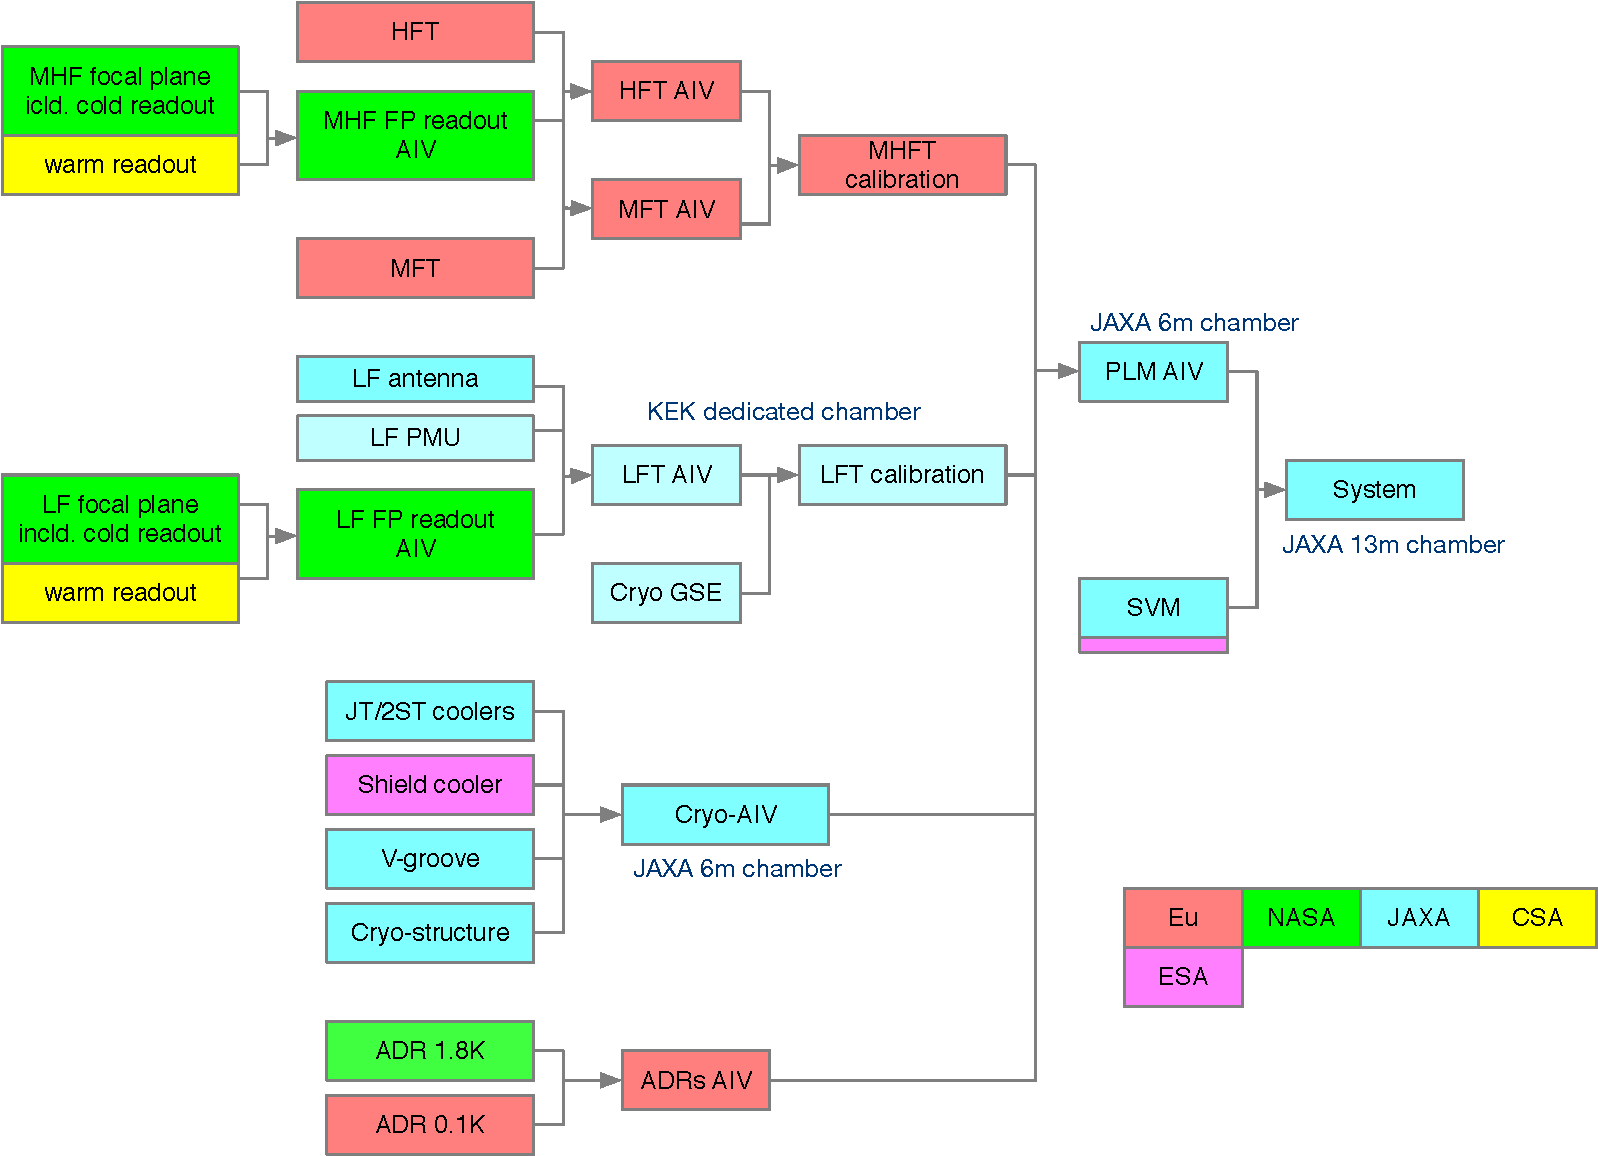
\includegraphics[width=12cm]{BUS-SoW/Figures/integration-scheme.pdf}
    \caption{\red{ミッション部とバスシステムのインテグレーション計画。}}
    \label{fig:integration-scheme}
\end{figure}

\section{運用準備}

担当企業は,運用準備(運用文書,運用手順,運用訓練,運用に必要なツール,運用手順の検証・運用訓練に必要な総合シミュレータ開発等)に必要な各作業を行う.

\subsection{軌道上運用}

%(以下は探査ミッションの記述なので、そのままは使わない方が良い)宇宙観測ミッションでは,決められた衛星リソース・機能性能と運用制約の下で,安全かつ科学成果最大化のための運用・判断が求められる.リスクと成果のバランスはケースバイケースで変わるため、定義が困難であることから,軌道上運用の意思決定はJAXA責任で行う必要がある.そのために必要な解析や運用文書整備には,開発企業のリソースと技術的知見を最大限活用することとし,仕様書・契約書で定義された範囲において企業責任で行う.また,運用支援(追跡管制のオペレータ等)やインフラ運用支援についても同様である.
軌道上運用は、JAXAの責任で実施する。担当企業は、必要な解析や運用文書整備を行い、運用の支援(追跡管制のオペレータ等)を行う。

\subsection{軌道上初期運用}
初期運用は、L2に着いて定常観測を始めるまでを指す。
担当企業は、打上後の初期運用準備作業,JAXAの地上システムを用いた初期運用,および初期機能確認評価を実施する.

\subsection{射場作業}

射場への輸送及び輸送後の機能確認,ロケットへの搭載作業,打上げ運用(射場作業)を実施する.


% \subsubsection{異常時運用}
%衛星のサバイバビリティに致命的となり得る異常を自動検知し、自律的に安全モードに移行できること。また、地上支援なしに、xx日以上その状態を維持できること。安全モードから定常観測に復帰する際には、地上支援を前提にして良い。安全モードおよびその復帰時に、一定の期間、観測ができなくなることは許容する。


\section{提出文書}

担当企業は、以下の文書を作成して、JAXAに提出する(TBD)。

\begin{enumerate}
    \item 運用のための文書
    \item 試験および解析結果に関する文書
    \item 各種審査の審査対象文書および補助文書のうち、担当企業が作成することが適切なもの
    \item その他
\end{enumerate}


\end{document}
